\documentclass[a4paper,12pt]{article}

% Packages
\usepackage[utf8]{inputenc}
\usepackage[T1]{fontenc}
\usepackage[english]{babel}
\usepackage{geometry}
\usepackage{titlesec}
\usepackage{multicol}
\usepackage{graphicx}
\usepackage{listings}
\usepackage{amsmath}
\usepackage{xcolor}
\usepackage{hyperref}


% Page setup
\geometry{margin=1in}
\titleformat{\section}{\normalfont\Large\bfseries}{\thesection}{1em}{}
\titleformat{\subsection}{\normalfont\large\bfseries}{\thesubsection}{1em}{}
\titleformat{\subsubsection}{\normalfont\normalsize\bfseries}{\thesubsubsection}{1em}{}

% Title
\title{Takuzu Project}
\author{DAUSSY Fabio}
\date{December 2023}

\lstset{% general command to set parameter(s)
language=C,tabsize=5,extendedchars=true,
basicstyle=\small, % print whole listing small
keywordstyle=\color{blue}\bfseries,
% underlined bold black keywords
identifierstyle=, % nothing happens
commentstyle=\color{red}, % white comments
stringstyle=\ttfamily, % typewriter type for strings
showstringspaces=false} % no special string spaces

\newenvironment{definition}[0]%
{\par\textbf{Definition: }}%
{\par}


\begin{document}

\maketitle


\section{Introduction}

\subsection{What is the Takuzu ?}
Takuzu, also known as Binairo or Binary Puzzle, is a logic-based combinatorial puzzle game. The objective of the game is to fill a grid with either 0s or 1s according to certain rules. The grid is typically square, and the size can vary.

The rules for Takuzu are simple:
\begin{enumerate}
    \item Each row and each column must contain an equal number of 0s and 1s.
    \item No more than two similar numbers (0s or 1s) can appear consecutively in any row or column.
\end{enumerate}



The puzzle starts with a partially filled grid, and the player's task is to complete the grid while adhering to these rules. The challenge lies in deducing the correct placement of 0s and 1s based on the given clues and the constraints imposed by the rules.

Takuzu puzzles are popular as pencil-and-paper games and are also available in various puzzle books and online platforms. They offer a fun and engaging way to challenge one's logical reasoning and deduction skills.


\subsection{The Report}

The goal of this project was to implement a 
solver/generator of Takuzu grid. Throught this report, 
we will not see in detail how the game has been implemented, but I will discuss
about some algorithm I used instead of other. Or just explain what i  

\section{Tree Structure of the project}

    
    \begin{figure}
        \centering
        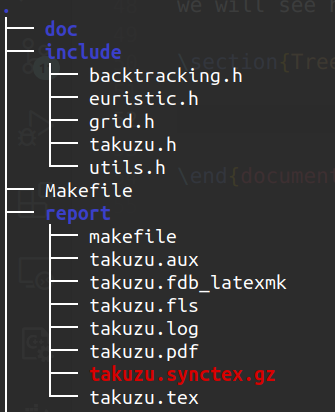
\includegraphics[scale=0.75]{img/tree1.png}
        \caption{Tree Structure}
    \end{figure}
    \begin{figure}
        \centering
        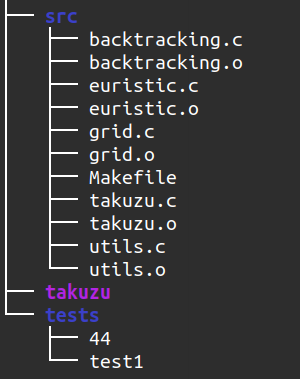
\includegraphics[scale=0.75]{img/tree2.png}
        \caption{Tree Structure 2}
    \end{figure}

    \begin{itemize}
        \item \textit{src} contains all the source files of the project
        \item \textit{include} contails all the headers used by the source files 
        \item \textit{report} contains all the files used to create this report
        \item \textit{tests} contains some grids to test with the program
        \item \textit{doc} contains all the instructions of the project given by the teacher.
        You can read the report and the associated assignment on the same time for a better understanding.
    \end{itemize} 

\section{Assignment 1}

The assignement 1 goal is to first create the tree structure of the project.
Followed by the creation of the main src (\textit{takuzu.c}). 
The first C code we wrote was the argument parser. 
To implement that, we used the POSIX function \textit{getopt\_long()}. 
Use ./takuzu -h to see all the details about the arguments and the options.
The interesting part in this assignment is how the options are stored in programs.
Some of my classmates chose to use a global structure. I didn't do that, 
I only used one global variable (the verbose). The other arguments are stored in the main function and if i need
one of them, I just pass them in the function parameters.
In addition, we set up a makefile to be more cumfortable with the compilation.

\section{Assignment 2}

In this assignment, We had to parse a file that represent a grid, and create the structure associated.
First, we created the structure of a grid in the \textit{grid.h} file: 
\\
    \begin{lstlisting}[language=C]
        typedef struct {
        int size;    // Number of elements in a row
        char** grid; // Pointer of the grid
    } t_grid;
    \end{lstlisting}
    
As you can see, I decided to use a pointer of pointer of char for the grid. I think it's more developper friendly even if I had to manage more malloc / free operations.


For the file\_parser, I used the POSIX function \textit{getline()}. The idea
was to parse the grid file line by line. It was possible because the pointer given by \textit{getline()} function 
is dynamic. So a line could be treated even if the line was very long.

\section{Assignment 3}

The assignment 3 ask to implement grid checking function and managing grid function. One of them is the \textit{grid\_copy()} function. Here we have just to be careful that we have to consider
that the destination grid parameter is not a NULL pointer. It permits to avoid dynamic allocation of the grid structure in addition of the content dynamic 
allocation of the grid structure.

About the verification of the grid, to check if two lines/columns are similar.
I wrote an algorithm that check the property:
\begin{equation}
    \forall i \in [1,n], j \in [i, n] \quad line_i \neq line_j 
\end{equation}
\begin{equation}
    \forall i \in [1,n], j \in [i, n] \quad col_i \neq col_j 
\end{equation}

This method avoid to repeat some comparisons, so we have a better complexity. For n the grid size :

\begin{equation}
    T(n) = n + (n-1) + (n-2)+ \dots + 2 + 1 = \frac{n(n+1)}{2}
\end{equation}

A little better than the naive one where $T(n) = n^2$

\section{Assignment 4}

\subsection{Heuristics}

This assignement required to implement the heuristics used to solve the grid.
I only added one more heuristics more than the ones explicited in the assignment statement.
\begin{itemize}
    \item The first heuristic says, if there are 2 consecutives 0 (resp. 1), the next and the previous cell will be 1 (resp. 0).
\end{itemize}

Basically, I just browse the grid and check if the property is verified and set the cell if it's the case.

\begin{itemize}
    \item  The second heuristic says, 
    if there is a line/column where the number of 0 (resp. 1) 
    is equal to $n/2$ (with n the grid size, even), the other empty cells of the line/column are 1s (resp. 0s)
\end{itemize}

To do that, I browse each line and each column, carrying 2 counters (count0 and count1). Verify the property with these counters and fill the empty cells whether it's true.

\begin{itemize}
    \item The last heuristic I added is, For an empty cell, if the cell to its left and to its right are 1 (resp. 0), the empty cell is a 0 (resp. 1)
    \item For an empty cell, if the cell to its top and to its bottom are 1 (resp. 0), the empty cell is a 0 (resp. 1)
\end{itemize}

Again, here, I just browse the grid and verify the property for each line and each column.

\subsection{Grid Generation}

Now we have to generate a random grid without verifying if it gets a solution. The main idea here is to generate a $N\%$ filled grid. 
To do that, we generate an empty grid of size $n$, 
and then compute the number of cells we have to fill to be at $N\%$ of filled cells. 
The number of cells to fill $k$ can be computed by the crosse product:
\begin{equation}
    k = \frac{n^2\times N}{100}
\end{equation}

Then, while the number of filled cell is lower than $k$, we randomly fill a cell and check whether the grid is consistent. If the grid isn't consistent after a filling, we undo it and fill an other cell.

\section{Assignment 5}

This is the interesting part! The \textbf{backtracking}! So, to solve a grid, we apply the maximum of heuristics on it. When we can't apply them anymore, we have to try several combination to solve the grid.

By using recursive functions, we manage to construct a binary tree that will compute all the possible combinations without making a C tree structure.
For example, for an unsolved grid $g$, we compute $g_1$ and $g_2$ where for a chosen empty cell $c$ on $g$: $g_1$ will set $c = 0$ and $g_2$ will set $c=1$. We repeat the operations for $g_1$, $g_2$, $g_{1_1}$, $g_{1_2}$, $g_{2_1}$, and so forth until the grid is valid or unconsistent (\ref{backtrack}).

\begin{figure}
    \centering
    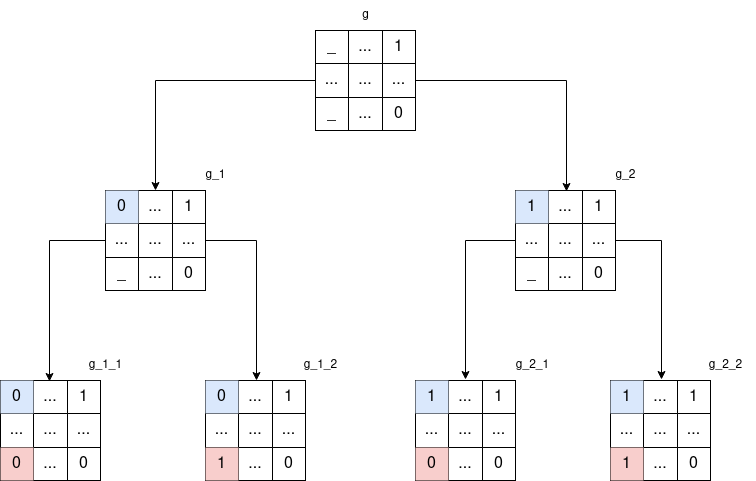
\includegraphics[scale=0.5]{img/tree.drawio.png}
    \caption{Backtracking example}\label{backtrack}
\end{figure}

I wrote two recursive function :
\begin{itemize}
    \item \textit{finsolution1}: find one solution and return it.
    \item \textit{findsolutionALL}: find all the possible solution of the grid and print them in the output file
\end{itemize}

They used the same principle. At the beginning we check if the parameter grid $g$ is valid or unconsistent. If its valid we print the current grid $g$, it means it's a solution. if it's unconsistent we drop it (\textit{return;})
On the other case it means the grid is consitent but not valid. 
So we choose an empty cell $c$ on the grid with the maximum weight (\ref{weig}). Then we create $g_1$ and $g_2$,
set $c$ to $0$ for $g_1$ and $c$ to $1$ for $g_2$ and call back the function to $g_1$ and $g_2$ respectively.

I use the weight to choose the cell to fill because if you fill an empty cell near non-empty cells, the heuristics have more chance to be applied in the next call.


\begin{definition}
    We define the \textbf{weight} $w: (i,j) \in [1,n]^2 \Longrightarrow [0,8]$ of a cell, the number of 0s and 1s around the cell. (Example \ref{wex})
\end{definition}\label{weig}

\begin{figure}
    \centering
    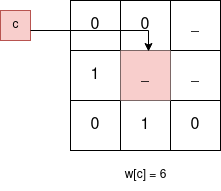
\includegraphics[scale=0.75]{img/weight.drawio.png}
    \caption{Weight of the cell c}\label{wex}
\end{figure}



\section{Assignment 6}

This last assignment consists of the creation of this report and the generation of a grid with one or several solutions.
I didn't look so far to implement it. I just make a loop that create random grid. If an unique solution is required, I regenerate a grid evertime if there is no exactly one solution (very very long). If multiple solution is autorized, I regenerate a grid if it doesn't have solution, when I found one, I stop.

\section{Conclusion}

It was a very interesting project, even if already manipulate C because we saw a lot of notions (error managing, getopt, backtracking...).
 But I very liked the last assignment with the backtracking because that was notion I didn't really implemented. It's scary but finally it's not that hard.
I also prefered the last part because we had more liberty of the way we could programs. I prefer the project where we only have one assignment and we are free
to implement it how we want. But I also understand the constraints of a bounded project because it was for beginner in C langage.

In conclusion, my project works! Great! Is it efficient, I think I could do better (recursion without allocating new grid) but some heuristics programming make my project, I think, actually efficient.
I hope you liked it!

\end{document}
